\chapter{Introduzione al corso}
%\addcontentsline{toc}{chapter}{Introduzione al corso}

Come avrai notato il titolo di questo libro è "Sistemi Operativi 1", questo perché il corso è diviso in due moduli.
In particolare in questo corso verranno affrontati i seguenti argomenti: gestione dei processi; scheduling dei processi; gestione della memoria principale; gestione della concorrenza tra processi; gestione del deadlock; gestione dell'input/output; gestione dei file system; nozioni basilari di sicurezza.\\\\
Possiamo immaginare i livelli di un computer come divisi in: \textit{Hardware}, utilizzato dagli sviluppatori dei sistemi operativi; \textit{Sistema Operativo} e \textit{Utilities,} utilizzati dai programmatori; \textit{Applicazioni}, principale target di un normale utente.

%In particolare in questo corso verrà insegnato come fa un "computer" a funzionare? Com'è possibile che premendo un tasto sulla tastiera, io "produca" sullo schermo una lettera (se sto usando, ad esempio, un editor)? muovendo il mouse, io veda il cursore che si muove sullo schermo? cliccando con il mouse, io possa aprire un nuovo programma? mentre navigo con il browser, io possa velocemente passare a leggere le email o scrivere il codice di un programma, mentre in contemporanea scarico un file? Com'è possibile che io possa scrivere un programma in maniera "semplice" e poi eseguirlo in modo altrettanto "semplice"? Com'è possibile che io possa scrivere un programma ed eseguirne contemporaneamente 2 istanze? La risposta corta è "perché c'è un sistema operativo". La risposta un po' più lunga e precisa è "perché c'è un sistema operativo che interagisce con l’hardware".
\begin{redbar}
    Quindi cosa fa effettivamente un \textbf{sistema operativo}? Il suo scopo primario è fornire un insieme di servizi sia per gli sviluppatori che per gli utenti dialogando e gestendo le risorse hardware.    
\end{redbar}
I principali servizi offerti da un sistema operativo sono: esecuzioni di programmi (app e servizi); fornire l'accesso ai dispostivi di input/output; accesso al sistema operativo stesso (shell); sviluppo di programmi (compilatori, editor e debugger); rilevamento e reazione ad errori; accounting (tutte le azioni che registrano, misurano e documentano le risorse concesse ad un utente); gestione delle risorse (può concedere il controllo del processore ad altri programmi).

Quindi un sistema operativo è un programma, il primo programma che va in esecuzione all'accensione della macchina, il cui scopo principale è controllare l'esecuzione degli altri programmi. Nel fare questo deve essere efficiente, conveniente e capace di evolvere.

Il \textit{kernel} (nucleo) è la parte del sistema operativo che si trova sempre in memoria principale, pronta per essere eseguita, e contiene le funzioni più usate. Nei moderni sistemi operativi si differenziano i kernel \textit{monolitici} e \textit{microkernel}. Nel primo tutte le parti del sistema operativo vengono caricate in memoria all'accensione del computer, mentre nel secondo, solo una minima parte del kernel è in memoria, il resto viene caricato quando serve.


%\begin{figure}[h]
%    \centering
%    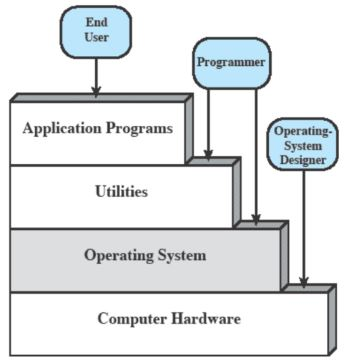
\includegraphics[width=0.3\linewidth]{images/strati-computer.JPG}
%    \caption{Livelli di un computer}
%    \label{fig:strati-computer}
%\end{figure}


\section{Componenti di un computer mono-processore}

\begin{wrapfigure}{r}{0.33\linewidth}
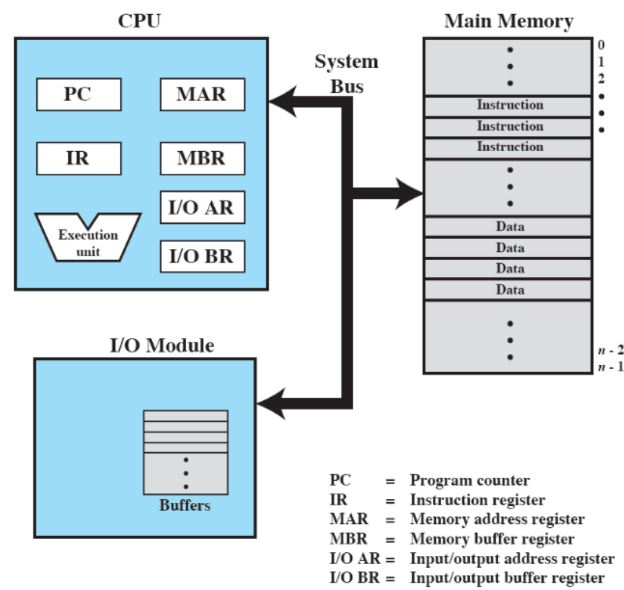
\includegraphics[width=1\linewidth]{images/computer-monoprocessore.JPG}
    %\caption{Architettura del computer}
    \label{fig:computer-monoprocessore}
\end{wrapfigure}

Un computer è formato da: una \textit{CPU} detta anche processore che contiene dei registri fondamentali per l'esecuzione di programmi; una RAM o \textit{memoria principale} volatile; dei \textit{dispositivi di input e output} (comprendono dispositivi di memoria secondaria non volatile, dispositivi per la comunicazione, tastiera, monitor, mouse...). Queste componenti devono poter comunicare tra loro e lo fanno attraverso i BUS di sistema.

I registri del processore si dividono in due macro-categorie: i registri visibili al programmatore che sono fondamentali per eseguire alcune istruzioni o per ridurre gli accessi alla memoria principale; i registri non visibili che sono utilizzati per controllare l'uso del processore stesso o per comunicare con la memoria e i dispositivi di I/O.\\\\
Un sistema operativo si basa sul concetto che di per sé un computer "sa fare" solo una cosa: \textit{fetch} e \textit{execute} di istruzioni milioni di volte. Ovvero, nella fase di fetch, il processore preleva il contenuto del Program Counter da cui ottiene un indirizzo, il cui contenuto viene inserito nell'Instruction Register; nella fase di execute, prende il contenuto dell'IR e lo esegue dopo aver incrementato il valore del PC.

\begin{Example}{Esecuzione di un programma}{}
    \textit{Vediamo un esempio di esecuzione di un programma con delle istruzioni a 16 bit di cui i primi 4 rappresentano l'Opcode mentre gli ultimi 12 l'Address. Con Opcode 0001 otteniamo una load, con 0010 una store, con 0101 un'add.}\\

    \begin{minipage}{\textwidth}
        \centering
        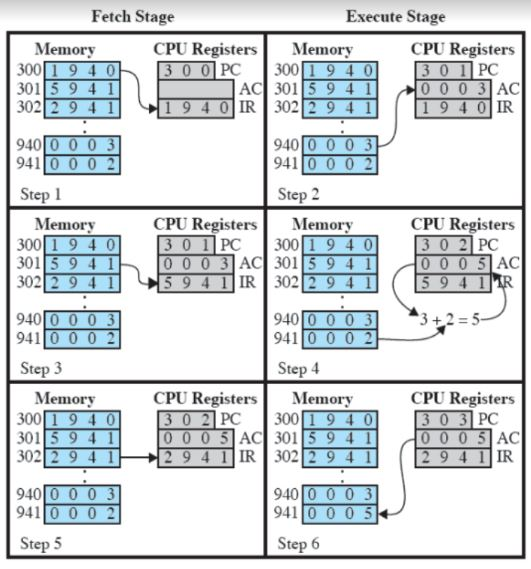
\includegraphics[width=0.5\linewidth]{images/esempio-esecuzione.JPG}
        \captionof{figure}{Esempio di esecuzione di un programma}
        \label{fig:esempio-esecuzione}
    \end{minipage}
    \\\\Notiamo come la RAM, a partire dall'indirizzo 300 contiene un mini-programma di 3 istruzioni. Nella prima fase di fetch viene inserito nell'IR l'istruzione 1940 e viene incrementato il PC, successivamente, dato che i primi quattro bit dell'istruzione (0001) rappresentano una load, viene caricata dalla memoria il valore contenuto nell'indirizzo 940 e inserito nel registro temporaneo AC. Nella seconda fase l'Opcode dell'istruzione risulta un'add (0101) che viene effettuata tra il valore in AC e il valore contenuto all'indirizzo 941. Infine viene effettuata una store all'indirizzo 941 del contenuto attuale di AC.
\end{Example}

\section{Interruzioni}
Un argomento fondamentale dell'interazione tra hardware e software sono le interruzioni. 
\begin{redbar}
    Un'\textbf{interruzione} (interrupt) ha il compito di interrompere la normale esecuzione del processore deviando l'esecuzione del processo ed eseguendo un software di sistema che fa parte del sistema operativo. 
\end{redbar}
Le interruzioni si dividono in due classi: interruzioni \textit{sincrone} e interruzioni \textit{asincrone}. Le interruzioni da programma sono le uniche sincrone ovvero, vengono generate come immediata conseguenza di una certa istruzione e per i processori Intel vengono chiamate exception. Le interruzioni asincrone, invece, vengono tipicamente sollevate dopo l’istruzione che le ha causate e ne esistono di vari tipi: le interruzioni da input/output vengono generate dal controllore di un dispositivo di I/O e segnalano il completamento o l'errore di un'operazione di I/O; le interruzioni da fallimento hardware sono le più imprevedibili in quanto vengono generate da errori relativi all'hardware; interruzioni da comunicazione tra CPU utilizzate per gestire la comunicazione tra più CPU; interruzioni da timer sono generate da un timer all'interno del processore e permettono al sistema operativo di effettuare delle operazioni ad intervalli regolari. 

Per le interruzioni asincrone, una volta che l’\textit{handler} (gestore di interruzioni) è terminato, si riprende dall'istruzione subito successiva a quella dove si è verificata l’interruzione. Quindi ad ogni ciclo fetch-execute, viene anche controllato se c'è stata un’interruzione. Se così fosse, il programma viene sospeso e viene eseguita una funzione che gestisce l’interruzione (interrupt-handler routine).
\begin{figure}
    \centering
    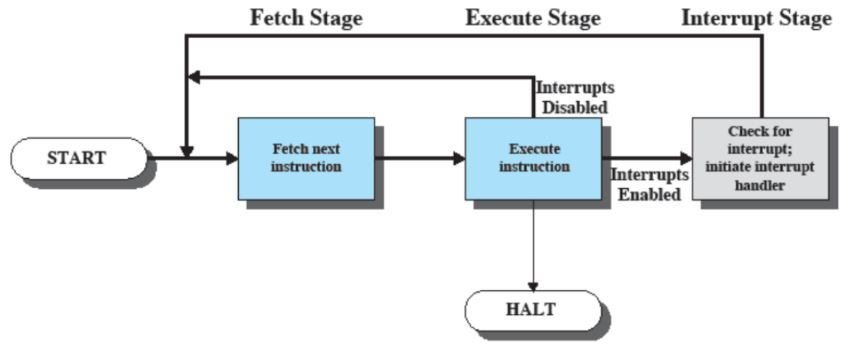
\includegraphics[width=0.70\linewidth]{images/fase-interrupt.JPG}
    \caption{Esecuzione di istruzioni con interruzioni}
    \label{fig:fase-interrupt}
\end{figure}
Nel punto in cui avviene questa "chiamata", il programma utente non prevedeva affatto di effettuare la chiamata all’interrupt-handler quindi è necessario che il sistema operativo e hardware collaborino per salvare le informazioni.

\begin{Example}{Gestione delle interruzioni}{}
    \textit{Il processore sta eseguendo l’istruzione all’indirizzo N quando arriva un’interruzione, da gestire con l’handler all’indirizzo Y.}
    
    \vspace{5pt}
    \begin{minipage}{0.4\textwidth}
        \vspace{0pt}
      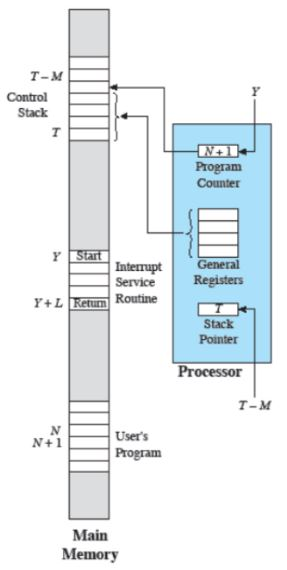
\includegraphics[width=\textwidth]{images/esempio-interrupt.JPG}
      %\captionof{figure}{Esempio di interruzioni in un programma}
    \end{minipage}
    \hspace{10pt}
    \begin{minipage}{0.55\textwidth}
        Nel momento in cui viene emessa l'interruzione il processore finisce di eseguire l'istruzione $N$, riconosce il segnale dell'interruzione, inserisce \textit{PSW}\footnote{Program Status Word è un registro speciale presente in un processore che contiene informazioni sullo stato attuale dell'esecuzione del programma.} e PC dentro il \textit{Contol Stack}, carica il nuovo PC in base all'interrupt ($Y$). Una volta eseguite le istruzioni dell'\textit{Interrupt Service Routine} viene ripristinata la memoria dei registri e del PC e si passa all'esecuzione dell'istruzione $N+1$.
    \end{minipage}
\end{Example}

In alcuni casi si possono generare più interrupt dando vita ad interrupt \textit{sequenziali} se gestiti uno dopo l'altro o interrupt \textit{annidati} quando un'interrupt ne genera altri.

\section{Miglioramento degli accessi}\label{sec:miglioramento-accessi}
Il più vecchio modo di gestire la comunicazione con i dispositivi di I/O veniva effettuata nel seguente modo: la CPU manda al dispositivo un comando; la CPU aspetta una riposta con un ciclo; la CPU effettua il trasferimento e la scrittura in memoria. Notiamo come questo processo è molto inefficiente in quanto completamente controllato da una CPU che nella maggior parte dei casi aspetta una risposta dal dispositivo. Un primo miglioramento lo troviamo con l'aggiunta delle interruzioni: si elimina il ciclo di attesa del processore in quanto è il dispositivo di I/O stesso a mandare l'interrupt una volta pronto. Nonostante questo notevole miglioramento c'è ancora un problema, la CPU deve ancora prendere il dato dai registri per poi scriverlo in memoria e ricompaiono le attese del processore quando si sovrappongono più richieste contemporaneamente. Per risolvere questi problemi viene sfruttato il \textit{DMA}\footnote{Direct Memory Access è quel meccanismo che permette di accedere direttamente alla memoria interna per scambiare dati, in lettura e/o scrittura, senza coinvolgere l'unità di controllo (CPU).}, generando un singolo interrupt per blocco trasferito e leggendo i dati direttamente dalla memoria, e la \textit{multiprogrammazione}, eseguendo più programmi contemporaneamente (la sequenza con cui i programmi sono eseguiti
dipende dalla loro priorità).

\section{Gerarchia della memoria}
Possiamo immaginare il mondo delle memorie come diviso in tre macro-categorie: \textit{Inboard Memory} comprende le memorie che si trovano direttamente sulla scheda madre del computer (Registri, Cache, Memoria principale); \textit{Outboard Storage} rappresenta le memorie che si trovano sui dispositivi di input/output (Dischi magnetici, CD, DVD, Penne USB...); \textit{Off-line Storage} riguarda quei dispositivi che si trovano al dì fuori del computer.

\begin{wrapfigure}{l}{0.40\linewidth}
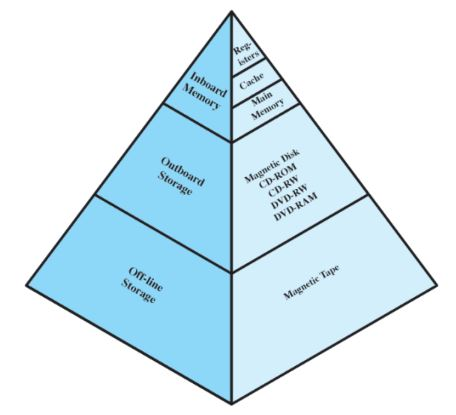
\includegraphics[width=1\linewidth]{images/gerarchia-memoria.JPG}
    \caption{Gerarchia della memoria}
    \label{fig:gerarchia-memoria}
\end{wrapfigure}

Seguendo la Figura \ref{fig:gerarchia-memoria} dall’alto verso il basso: diminuisce la velocità di accesso; diminuisce il costo al bit; aumenta la capacità; diminuisce la frequenza di accesso alla memoria da parte del processore.

La CPU normalmente accede molto spesso alla memoria volatile della Inboard Memory e raramente alle memorie secondarie (Outboard e
Offline Storage).

Anche nell’Inboard Memory ci sono importanti differenze di velocità, infatti, la velocità del processore è maggiore della velocità di accesso alla memoria principale. Per evitare eccessivi tempi di attesa, tutti i computer hanno una memoria \textit{cache} che contiene copie di porzioni della memoria principale e che sfrutta il principio di \textit{località dei riferimenti}\footnote{E' la tendenza di un processore ad accedere ripetutamente allo stesso insieme di posizioni di memoria in un breve periodo di tempo.}. Quando la CPU vuole leggere un indirizzo, se il blocco corrispondente è presente nella cache allora il dato viene caricato (\textit{HIT}), altrimenti il dato viene preso dalla RAM e il blocco copiato nella cache (\textit{MISS}) attraverso una funzione di mappatura. Invece quando un dato deve essere sovrascritto si utilizza generalmente la politica di rimpiazzo LRU\footnote{Least Recently Used, si rimpiazza il blocco usato meno di recente.} e la memoria principale si può aggiornare in due modi: tramite il \textit{Write Through} dove ad ogni modifica viene aggiornato il blocco in memoria; con il \textit{Write Back} dove il blocco viene aggiornato solo quando viene sostituito.

\section{Storia dei sistemi operativi}
Nel corso della storia i sistemi operativi hanno attraversato diverse fasi "evolutive" che è importante conoscere per capire gli schemi che sono stati utilizzati per l'aggiornamento dell'hardware, aggiunta di nuovi servizi o correzione di errori.

Negli anni '40 non c'era nessun sistema operativo e venivano utilizzati degli interruttori per l'input e delle stampanti per gli output. Quasi fin da subito gli input furono migliorati attraverso delle schede perforate con un tipo di computazione prettamente seriale. 

Il primo sistema operativo nacque quando si iniziarono ad inserire più programmami da eseguire chiamati \textit{jobs} e un loro particolare linguaggio di controllo. Questo sistema funzionava particolarmente bene per i sistemi \textit{batch} (non interattivi). Tutto ciò iniziò a mettere in luce delle necessità a cui bisognava iniziare a pensare: \textit{protezione della memoria} per prevenire eventuali riscritture di codice da parte di un job; \textit{timer} per impedire l'enorme esaurimento di tempo da parte di alcuni job; \textit{istruzioni privilegiate} per permettere al sistema di controllo dei job di effettuare operazioni più alte. Così, come avviene tuttora, si passò ad eseguire i job solo in modalità \textit{utente}, bloccando l'accesso ad alcune funzioni, e i monitor in modalità \textit{sitema} (o kernel) permettendo l'utilizzo di istruzioni privilegiate o l'accesso ad aree protette della memoria.

Nonostante ciò, più del 96\% del tempo della CPU era sprecato ad aspettare i dispositivi di I/O. Si iniziò a pensare alla \textit{multiprogrammazione} eseguendo più programmi contemporaneamente durante i tempi di attesa dei processi migliorando di gran lunga le prestazioni del sistema operativo. 

A partire dagli anni '60 la richiesta di job interattivi iniziò a diventare sempre più esigente. Ogni utente infatti era collegato, tramite un terminale, ad un unico grande computer (main frame), e si iniziarono a sviluppare dei sistemi di condivisione del tempo (\textit{Time Sharing System}), dove il tempo del processore era condiviso tra più utenti.

Tutto questo portò ad ulteriori sviluppi interessanti che sono tutt'ora validi per i sistemi operativi: il concetto di processo; la gestione della memoria; sicurezza e protezione delle informazioni (privacy); gestione dello scheduling e delle risorse;
strutturazione del sistema.

Il \textit{processo} riunisce in un unico concetto il job non-interattivo e quello interattivo ed è un’unità di computazione caratterizzata da: almeno un flusso di esecuzione (thread); uno stato corrente; un insieme di risorse di sistema ad esso associate.

Quando si parla invece di strutturazione del sistema si intende raggruppare insieme delle funzioni analoghe in livelli.